\documentclass[final]{beamer}
  \mode<presentation>
  {
% you can chose your theme here:
\usetheme{ssc2014}
% further beamerposter themes are available at 
% http://www-i6.informatik.rwth-aachen.de/~dreuw/latexbeamerposter.php
}
  \usepackage{type1cm}
  \usepackage{calc} 
  \usepackage{times}
  \usepackage{wrapfig}
  \usepackage[labelformat=empty]{caption}
  \usepackage{amsmath,amsthm, amssymb, latexsym}
  \boldmath
  \usepackage[english]{babel}
  \usepackage[latin1]{inputenc}
  \usepackage[orientation=landscape,width=71, height=35,debug]{beamerposter}
  
  \setbeamertemplate{caption}{\insertcaption} \setbeamertemplate{caption label separator}{}
  
  \title{SSC 2014 Case Study Competition}
  \author{Sahir Bhatnagar, Kevin McGregor and Maxime Turgeon}
  \institute{Department of Epidemiology, Biostatistics and Occupational Health, McGill University} 
  \date{May 26, 2013}
  
\usepackage{environ}% Required for \NewEnviron, i.e. to read the whole body of the environment
\makeatletter

\newcounter{acolumn}%  Number of current column
\newlength{\acolumnmaxheight}%   Maximum column height


% `column` replacement to measure height
\newenvironment{@acolumn}[1]{%
    \stepcounter{acolumn}%
    \begin{lrbox}{\@tempboxa}%
    \begin{minipage}{#1}%
}{%
    \end{minipage}
    \end{lrbox}
    \@tempdimc=\dimexpr\ht\@tempboxa+\dp\@tempboxa\relax
    % Save height of this column:
    \expandafter\xdef\csname acolumn@height@\roman{acolumn}\endcsname{\the\@tempdimc}%
    % Save maximum height
    \ifdim\@tempdimc>\acolumnmaxheight
        \global\acolumnmaxheight=\@tempdimc
    \fi
}

% `column` wrapper which sets the height beforehand
\newenvironment{@@acolumn}[1]{%
    \stepcounter{acolumn}%
    % The \autoheight macro contains a \vspace macro with the maximum height minus the natural column height
    \edef\autoheight{\noexpand\vspace*{\dimexpr\acolumnmaxheight-\csname acolumn@height@\roman{acolumn}\endcsname\relax}}%
    % Call original `column`:
    \orig@column{#1}%
}{%
    \endorig@column
}

% Save orignal `column` environment away
\let\orig@column\column
\let\endorig@column\endcolumn

% `columns` variant with automatic height adjustment
\NewEnviron{acolumns}[1][]{%
    % Init vars:
    \setcounter{acolumn}{0}%
    \setlength{\acolumnmaxheight}{0pt}%
    \def\autoheight{\vspace*{0pt}}%
    % Set `column` environment to special measuring environment
    \let\column\@acolumn
    \let\endcolumn\end@acolumn
    \BODY% measure heights
    % Reset counter for second processing round
    \setcounter{acolumn}{0}%
    % Set `column` environment to wrapper
    \let\column\@@acolumn
    \let\endcolumn\end@@acolumn
    % Finally process columns now for real
    \begin{columns}[#1]%
        \BODY
    \end{columns}%
}
\makeatother

%\newlength{\myheight}

\begin{document}
  \begin{frame} 
    \vfill
    
        \begin{acolumns}[t]
          
          
          
          \begin{column}{.24\linewidth}
          
          
            \begin{block}{Abstract}
    			We consider the effect of economy on the amount of time Americans reported watching television on the ATUS  between 2003 and 2012. Measures of economic performance include GDP, unemployment rate, and stock indices; these measures are summarized using their first two principal components. A GLM is used to test the association between economy and TV time use, with time being included smoothly. We report that watching television is associated with both PCs, and that the association changes with gender (but not with region, race or income). Then, using penalized regression, we determine that the strongest sociodemographic factors influencing television viewing are age, gender, presence of household children, and average number of hours worked in a week.  The stratified sampling scheme is accounted for through regression techniques, and two seperate models are used to deal with the zero-inflated nature of the data. 
            
            \end{block}
            
            \begin{block}{Main questions}
                        
                        \begin{enumerate}
                        	\item What effect does the economy have on the amount of time spent watching TV? Does this vary by gender, race, income? 
            
                        	\item What are the strongest socio-demographic predictors of time spent watching TV?
                        \end{enumerate}
                        \autoheight
                       \end{block}
            
          
          \end{column}
          
          \begin{column}{.24\linewidth}
            \begin{block}{Description of the data}
              \begin{itemize}
              	\item Since 2003, the American Time Use Survey (ATUS) has been collecting information on how Americans spend a day, what kind of activities they perform, with whom, and for how long.
              	\item Over a decade, some 135,000 respondents were asked to walk an interviewer through a selected day.
              	\item The dataset itself contains socio-demographic information about the respondents (e.g. sex, race, income), as well as time-use variables (e.g. sleeping, working, watching TV)
              \end{itemize}
              
            \end{block}
    
          
          
          \begin{block}{Main challenges}
                  		  \begin{itemize}
                  		  	\item About 20\% of respondents reported no TV watching; two separate models are used to address this issue
                  		  	
                  		  	\item How can economy be measured? \textbf{Note}: economy cannot have a direct, causal effect on TV watching
                  		  	
                  		  	\item Since economy varies with time, how can we separate the effect of time from the effect of economy?
                  		  	
                  		  	\item How to take into account the stratified sampling scheme?
                  		  	\begin{itemize}
                  		  		\item Through regression (Gelman, 2007)
                  		  	\end{itemize}
                  		  	
                  		  	\item How to handle missing data
                  		  \end{itemize}
                  			
                            \autoheight 
                          \end{block}
                          
                        
        \end{column}
                        
          
        
    
  
              \begin{column}{.48\linewidth}
              
                
             
                \begin{block}{Economic measures and Distribution of TV use}
                	
                 \begin{figure}
                 \centering
                 
                 \begin{minipage}{0.5\textwidth}
                 \centering
                 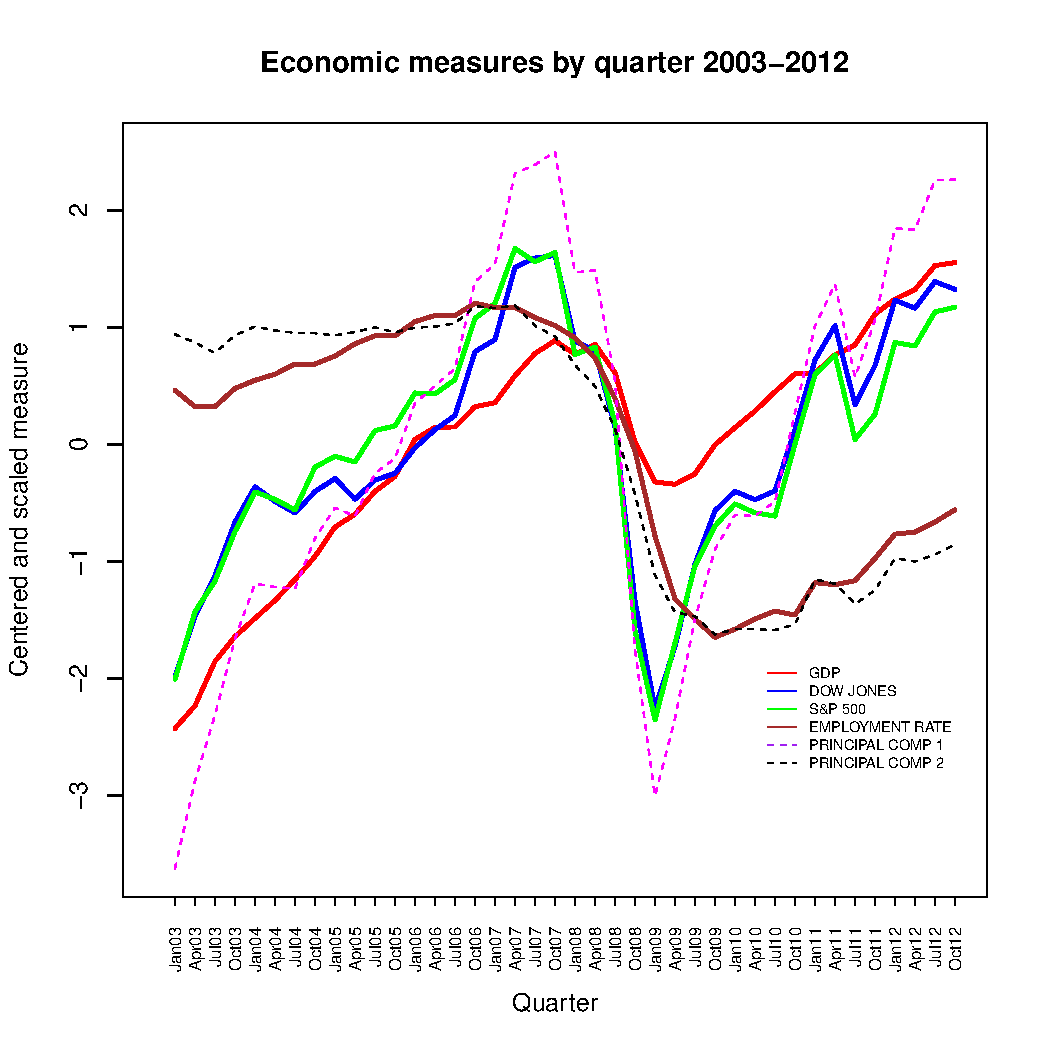
\includegraphics[width=.75\textwidth]{econ_measures.pdf}
                 \end{minipage}%                 
                 \begin{minipage}{0.5\textwidth}
                 \centering
                 \begin{figure}
                 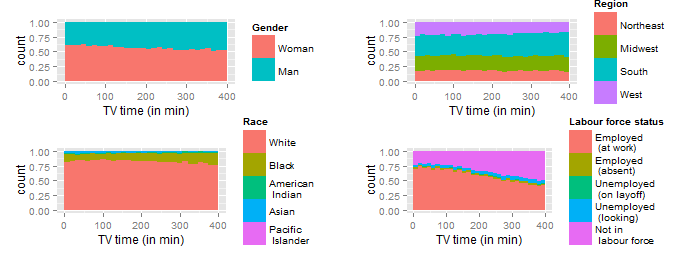
\includegraphics[height=0.25\textheight,width=\textwidth]{stratification}
                 \caption{Reported TV time, stratified according to gender, race, region, and labour force status}
                 \end{figure}
                 \end{minipage}%                 
                 \end{figure}
                                 
                \autoheight
               \end{block}
               
             
               \end{column}
              
            \end{acolumns}
        
        
        \vfill
    
    \begin{acolumns}[t]
    
    \begin{column}{.72\linewidth}
    \begin{center}
   		\LARGE{1. Effect of economy}
    \end{center}
     \begin{block}{Methods}
       
       To test for the effect of economy, we use two GLMs: gamma regression and logistic regression.
       $$g(\mu_i)=\beta_1ECON1_i+\beta_2ECON2_i + \alpha^t X_i + \lambda(t_i),$$
       where $X_i$ are the covariates accounting for the stratified sampling scheme (gender, day of the week, region, hispanicity, race) and $\lambda(t)$ is a smooth function of time (measured in months). The smoothing was done via linear extrapolation:
       $$E\left(\lambda(t)|\lambda(t-1),\lambda(t-2),\ldots,\lambda(1)\right) = 2\lambda(t-1) - \lambda(t-2).$$
       The stochastic part of the models are respectively
       $$TVTIME_i\sim \mathrm{Gamma}(\nu, \lambda_i),\hspace{1cm} g(x)=\log(x),\qquad\mbox{and}\qquad TVIND_i\sim \mathrm{Bernouilli}(\pi_i), \hspace{1cm} g(x)=\mathrm{logit}(x).$$
       The model was fitted using Gibbs sampling, via JAGS (Plummer, 2003) and \texttt{R}, using a 10\% random sample.
        
     \end{block}
     
     
     \begin{block}{Results}
     
     \begin{figure}
      \centering                      
      \begin{minipage}{0.25\textwidth}
      \centering
      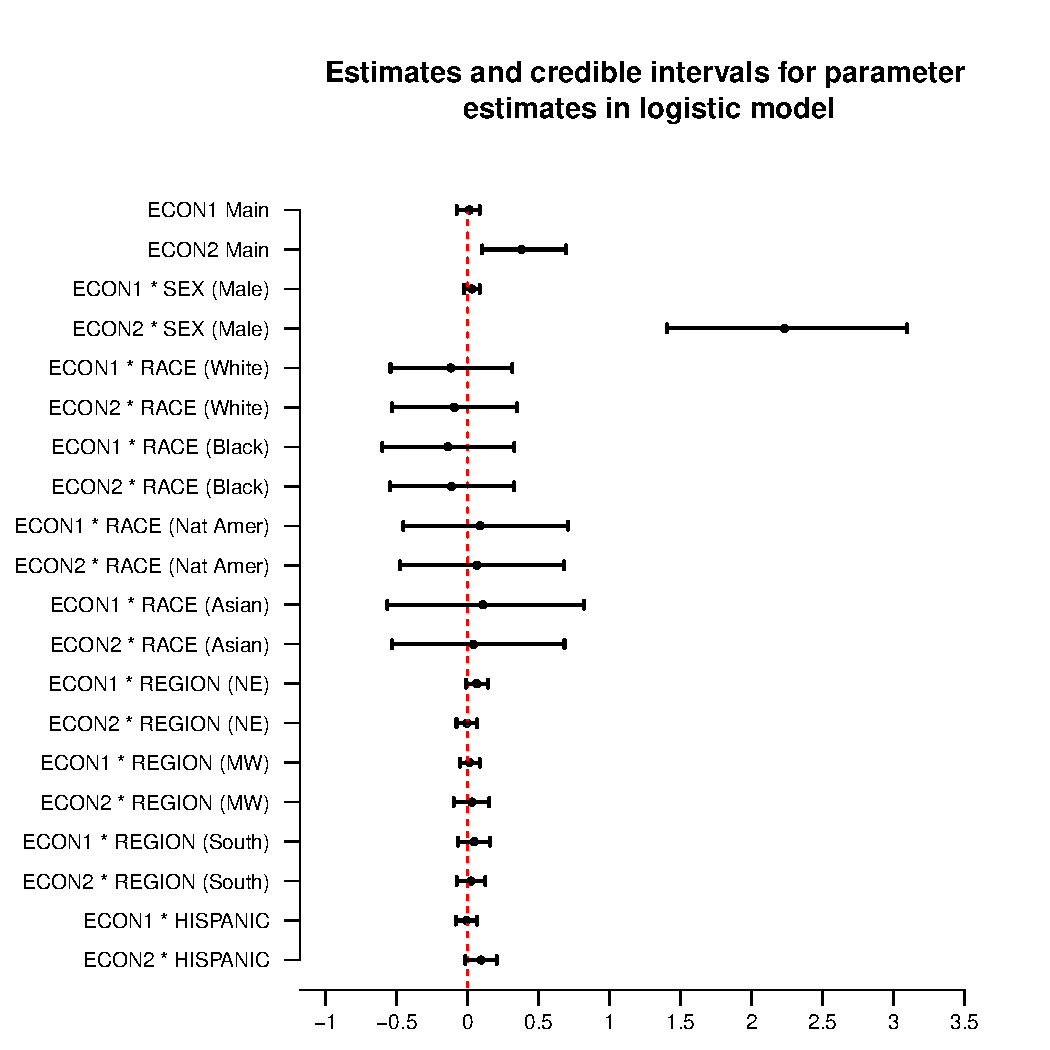
\includegraphics{logit_estimates.pdf}
      \end{minipage}%   
      \begin{minipage}{0.25\textwidth}
             \centering
             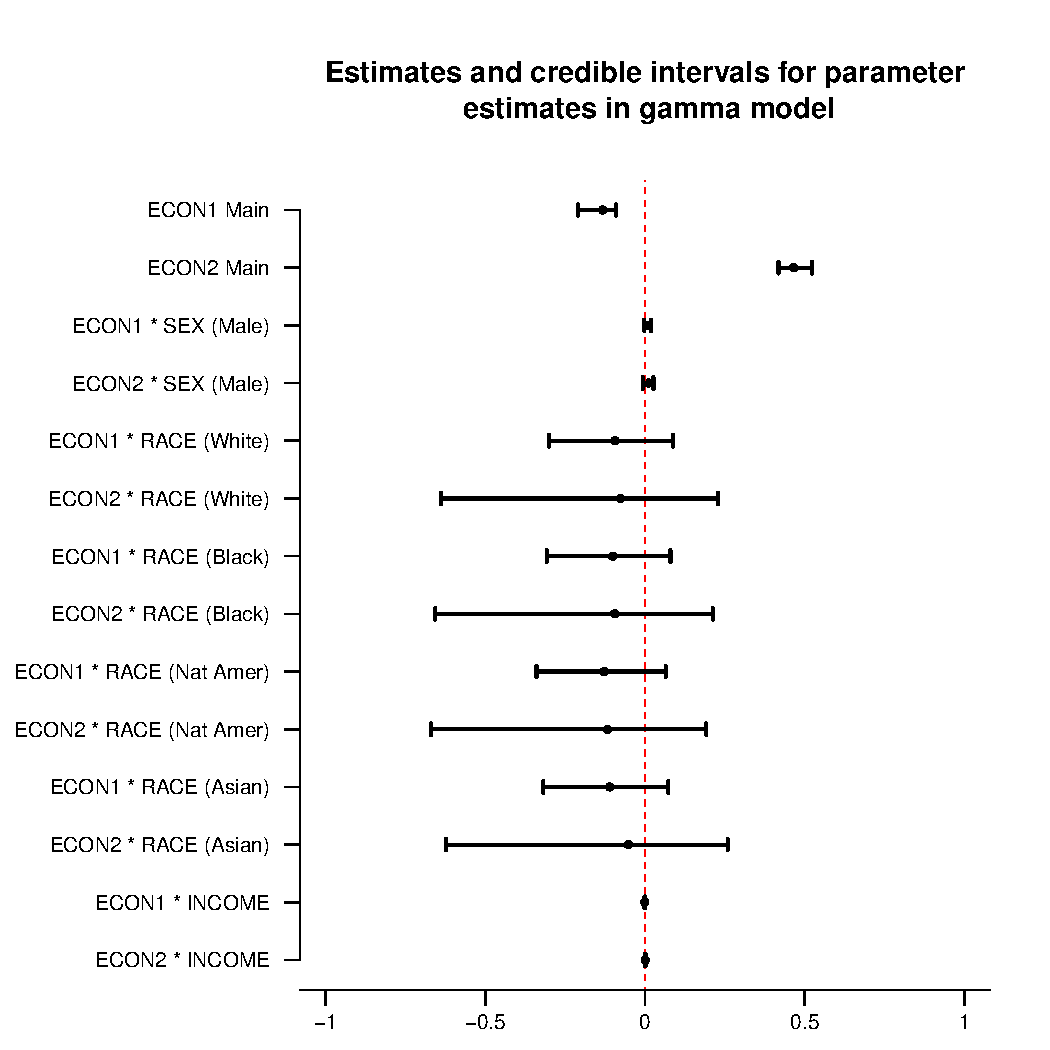
\includegraphics{gamma_estimates.pdf}
            \end{minipage}%                    
      \begin{minipage}{0.25\textwidth}
      \centering
      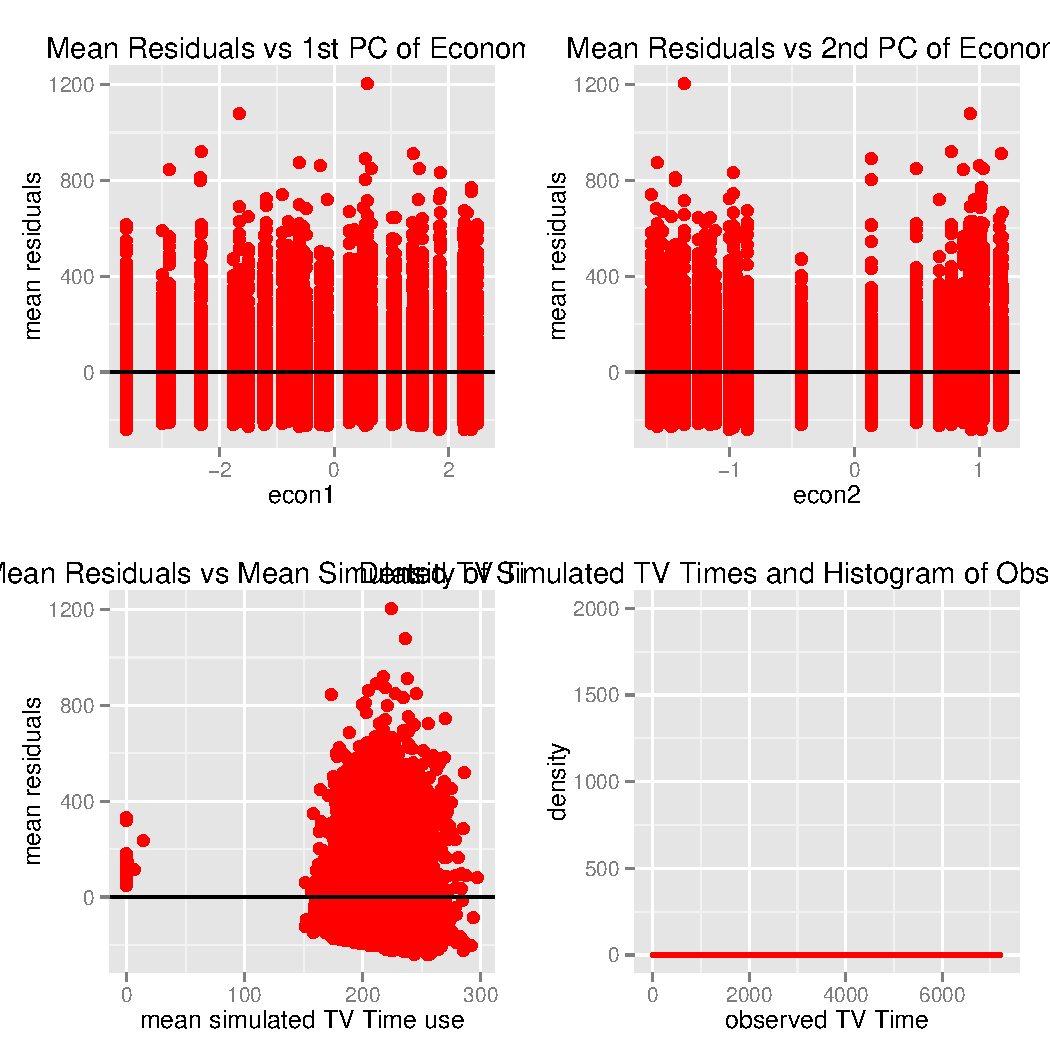
\includegraphics{validation.pdf}
      \caption{Model diagnostics}
      \end{minipage}%      
      \begin{minipage}{0.25\textwidth}
       \centering
       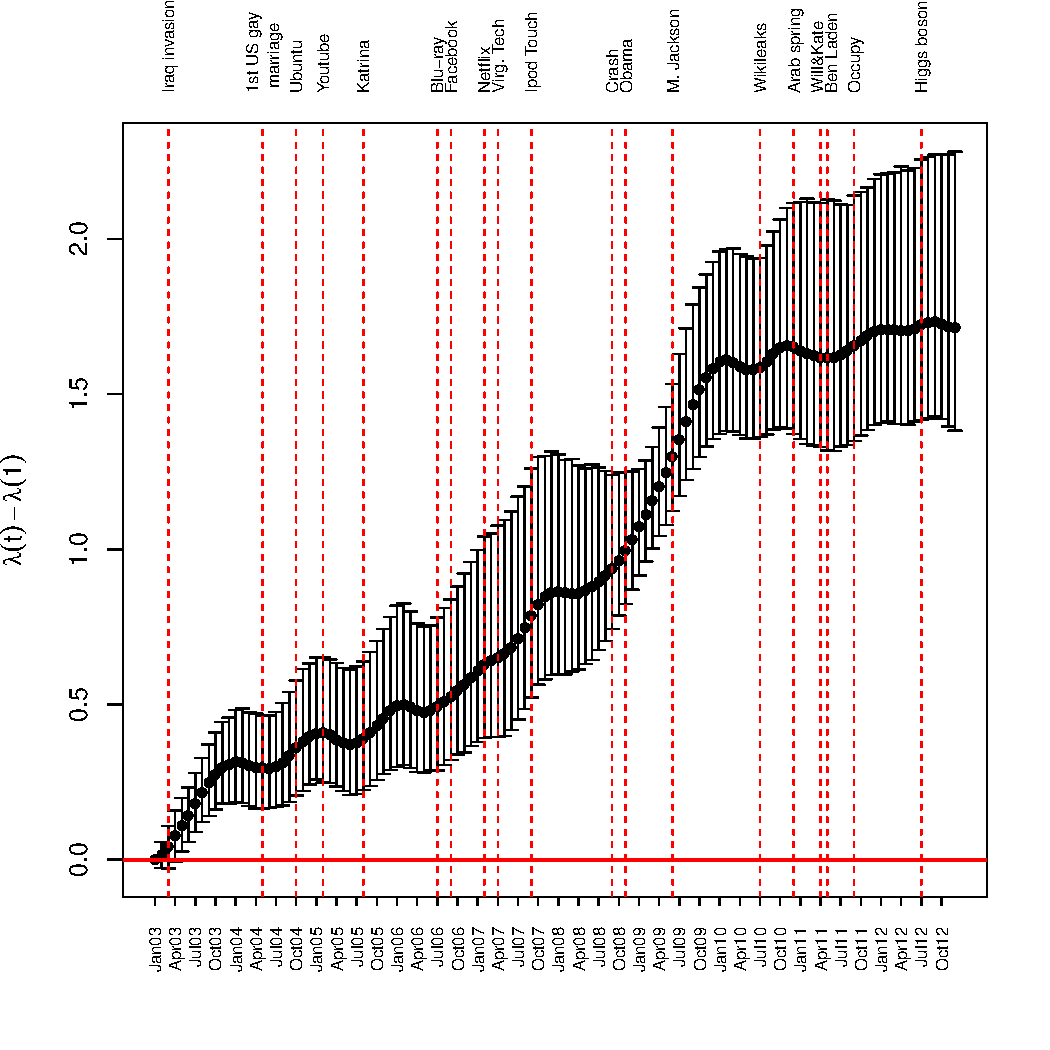
\includegraphics{time_trend.pdf}
       \caption{Smoothed time trend and major events}
      \end{minipage}%            
                      
      \end{figure}
     
          
       
      \autoheight 
     \end{block}
     
                     
    \end{column}
              
    
    \begin{column}{.24\linewidth}
    \begin{center}
    	\LARGE{2. Main socio-demographic predictors}
    \end{center}
    
    \begin{block}{Socio-demographic variables}
                    \begin{itemize}
                    	\item Gender, age, region, race, hispanicity, marital status, education level, presence of household children or spouse, US citizenship status
                    	
                    	\item Weekly earnings, labour force status, number of jobs, average number of hours worked in a week
                    	
                    	\item Month and year the interview was conducted, the day of the week, whether it was a holiday
                    	
                    \end{itemize}
                                 
                    
                   \end{block}
                      
                  
    
     \begin{block}{Methods}
     	\begin{itemize}
     		\item We use a penalized GLM to select the most relevant socio-demographic factors. The group-Lasso penalty (Yuan \& Lin, 2007) is:
     		$$\tau \sum_{\ell=1}^{L}\sqrt{p_\ell}\|\beta_\ell\|_2.$$
     		This penalty is used to account for the fact that some predictors are categorical. Here, $p_\ell$ is the number of features in group $\ell=1,\ldots,L$.
     		\item The tuning parameter $\tau$ is selected using 10-fold cross-validation and the one-standard error rule (Hastie \emph{et al.}, \emph{Elements of Statistical Learning})
     	\end{itemize}
        
                     
     \end{block}
          
          
     \begin{block}{Results}
        \begin{itemize}
        	\item For the \textbf{logistic model}, the selected factors are: presence of household children, age, gender, average number of hours worked in a week, and the number of jobs.
        	
        	\item For the \textbf{gamma model}, the selected factors are: presence of household children, age, gender, weekly earnings, presence of spouse in household, average number of hours worked in a week, diary day, education level, race, and the number of jobs.
        \end{itemize}
       \autoheight                   
     \end{block}
     
        
    \end{column}
    
    
    \end{acolumns}
    
    \vfill
    
        \begin{acolumns}[t]
        
        \begin{column}{.24\linewidth}
        		
                 
                 \begin{block}{Discussion}
                 	\begin{itemize}
                 		\item \textbf{Why Bayesian}: convenient computational tools, smooth time effect, and exact inference
                 		
                 		\item \textbf{Survey weighting is overrated}: regression methods are sufficient
                 		
                 		\item \textbf{Zero inflation}: two phenomena, two models
                 		
                 		\item \textbf{Computational efficiency}: Group-Lasso fast, Gibbs sampling slow
                 	\end{itemize}
                  \autoheight   
                 \end{block}
                              
        \end{column}
        
        \begin{column}{.24\linewidth}
		
         
         \begin{block}{Strengths}
         	\begin{itemize}
         		\item The model is effectively separating the economic trend from the time trend
         		\item The measure of economy being used is quite flexible
         		\item The model was able to differentiate between the effect of unemployment and the effect of market behaviour
         	\end{itemize}
          \autoheight   
         \end{block}
                      
        \end{column}
                  
        
        \begin{column}{.24\linewidth}
         
         \begin{block}{Limitations}
         	\begin{itemize}
         		\item The gamma GLM assumes a constant dispersion parameter; model diagnostics seem to indicate otherwise
         		\item The model does not include the natural auto-regressive structure of the economic variables
         		\item The measure of association with economy may be too coarse
         		\item To measure economy, we used PCA, which ignores the relationship with the response
         	\end{itemize}
          \autoheight   
         \end{block}
                      
        \end{column}
        
        
         \begin{column}{.24\linewidth}
                 
          \begin{block}{Acknowledgements}
             \begin{center}
             We would like to thank Dr.~Celia~Greenwood, Dr. Olli~Saarela, Dr.~Abbas~Khalili, and Dr.~James~Hanley for their help and input on this project. The training and advice they have provided and continue to provide has been influential on this project and beyond.
             \end{center}
             
           \autoheight   
          \end{block}
                              
         \end{column}
        
        
        \end{acolumns}
    
    \vfill 
  \end{frame}
\end{document}
